\documentclass[1p]{elsarticle_modified}
%\bibliographystyle{elsarticle-num}

%\usepackage[colorlinks]{hyperref}
%\usepackage{abbrmath_seonhwa} %\Abb, \Ascr, \Acal ,\Abf, \Afrak
\usepackage{amsfonts}
\usepackage{amssymb}
\usepackage{amsmath}
\usepackage{amsthm}
\usepackage{scalefnt}
\usepackage{amsbsy}
\usepackage{kotex}
\usepackage{caption}
\usepackage{subfig}
\usepackage{color}
\usepackage{graphicx}
\usepackage{xcolor} %% white, black, red, green, blue, cyan, magenta, yellow
\usepackage{float}
\usepackage{setspace}
\usepackage{hyperref}

\usepackage{tikz}
\usetikzlibrary{arrows}

\usepackage{multirow}
\usepackage{array} % fixed length table
\usepackage{hhline}

%%%%%%%%%%%%%%%%%%%%%
\makeatletter
\renewcommand*\env@matrix[1][\arraystretch]{%
	\edef\arraystretch{#1}%
	\hskip -\arraycolsep
	\let\@ifnextchar\new@ifnextchar
	\array{*\c@MaxMatrixCols c}}
\makeatother %https://tex.stackexchange.com/questions/14071/how-can-i-increase-the-line-spacing-in-a-matrix
%%%%%%%%%%%%%%%

\usepackage[normalem]{ulem}

\newcommand{\msout}[1]{\ifmmode\text{\sout{\ensuremath{#1}}}\else\sout{#1}\fi}
%SOURCE: \msout is \stkout macro in https://tex.stackexchange.com/questions/20609/strikeout-in-math-mode

\newcommand{\cancel}[1]{
	\ifmmode
	{\color{red}\msout{#1}}
	\else
	{\color{red}\sout{#1}}
	\fi
}

\newcommand{\add}[1]{
	{\color{blue}\uwave{#1}}
}

\newcommand{\replace}[2]{
	\ifmmode
	{\color{red}\msout{#1}}{\color{blue}\uwave{#2}}
	\else
	{\color{red}\sout{#1}}{\color{blue}\uwave{#2}}
	\fi
}

\newcommand{\Sol}{\mathcal{S}} %segment
\newcommand{\D}{D} %diagram
\newcommand{\A}{\mathcal{A}} %arc


%%%%%%%%%%%%%%%%%%%%%%%%%%%%%5 test

\def\sl{\operatorname{\textup{SL}}(2,\Cbb)}
\def\psl{\operatorname{\textup{PSL}}(2,\Cbb)}
\def\quan{\mkern 1mu \triangleright \mkern 1mu}

\theoremstyle{definition}
\newtheorem{thm}{Theorem}[section]
\newtheorem{prop}[thm]{Proposition}
\newtheorem{lem}[thm]{Lemma}
\newtheorem{ques}[thm]{Question}
\newtheorem{cor}[thm]{Corollary}
\newtheorem{defn}[thm]{Definition}
\newtheorem{exam}[thm]{Example}
\newtheorem{rmk}[thm]{Remark}
\newtheorem{alg}[thm]{Algorithm}

\newcommand{\I}{\sqrt{-1}}
\begin{document}

%\begin{frontmatter}
%
%\title{Boundary parabolic representations of knots up to 8 crossings}
%
%%% Group authors per affiliation:
%\author{Yunhi Cho} 
%\address{Department of Mathematics, University of Seoul, Seoul, Korea}
%\ead{yhcho@uos.ac.kr}
%
%
%\author{Seonhwa Kim} %\fnref{s_kim}}
%\address{Center for Geometry and Physics, Institute for Basic Science, Pohang, 37673, Korea}
%\ead{ryeona17@ibs.re.kr}
%
%\author{Hyuk Kim}
%\address{Department of Mathematical Sciences, Seoul National University, Seoul 08826, Korea}
%\ead{hyukkim@snu.ac.kr}
%
%\author{Seokbeom Yoon}
%\address{Department of Mathematical Sciences, Seoul National University, Seoul, 08826,  Korea}
%\ead{sbyoon15@snu.ac.kr}
%
%\begin{abstract}
%We find all boundary parabolic representation of knots up to 8 crossings.
%
%\end{abstract}
%\begin{keyword}
%    \MSC[2010] 57M25 
%\end{keyword}
%
%\end{frontmatter}

%\linenumbers
%\tableofcontents
%
\newcommand\colored[1]{\textcolor{white}{\rule[-0.35ex]{0.8em}{1.4ex}}\kern-0.8em\color{red} #1}%
%\newcommand\colored[1]{\textcolor{white}{ #1}\kern-2.17ex	\textcolor{white}{ #1}\kern-1.81ex	\textcolor{white}{ #1}\kern-2.15ex\color{red}#1	}

{\Large $\underline{12a_{0394}~(K12a_{0394})}$}

\setlength{\tabcolsep}{10pt}
\renewcommand{\arraystretch}{1.6}
\vspace{1cm}\begin{tabular}{m{100pt}>{\centering\arraybackslash}m{274pt}}
\multirow{5}{120pt}{
	\centering
	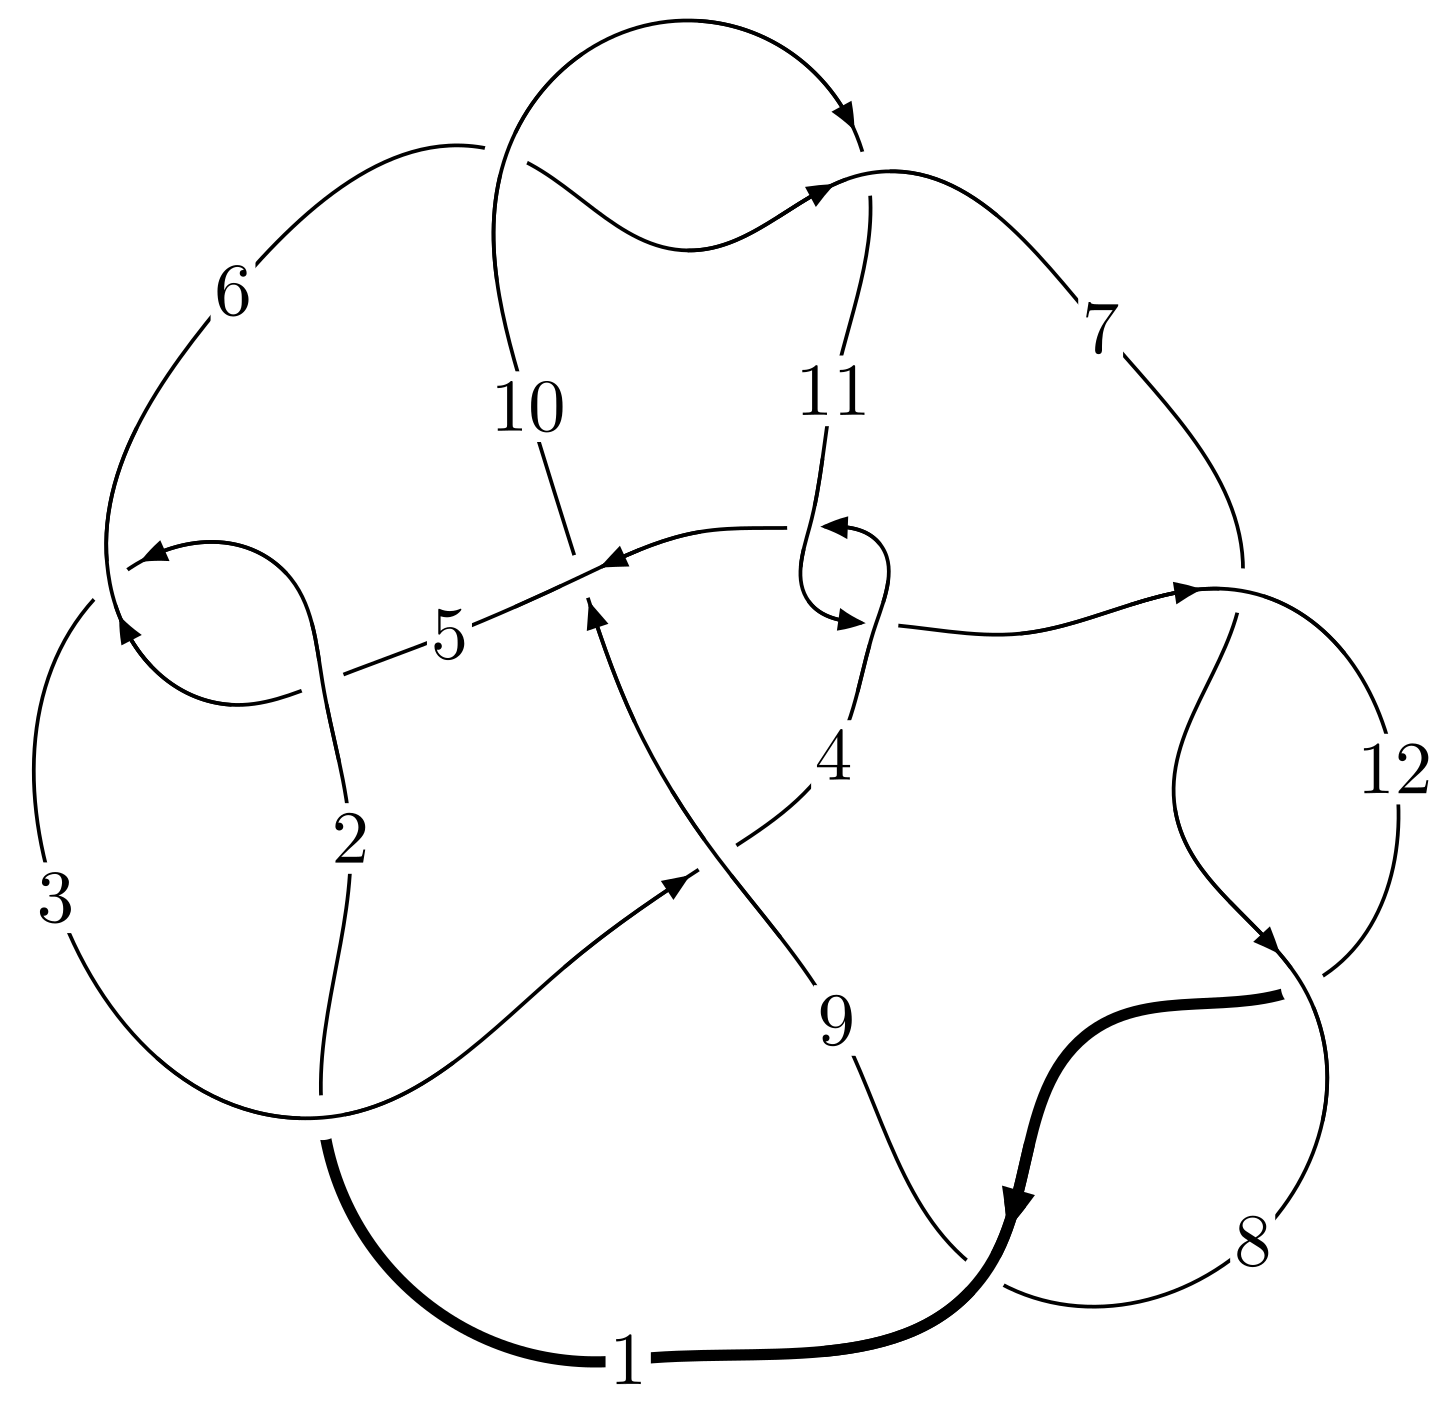
\includegraphics[width=112pt]{../../../GIT/diagram.site/Diagrams/png/1195_12a_0394.png}\\
\ \ \ A knot diagram\footnotemark}&
\allowdisplaybreaks
\textbf{Linearized knot diagam} \\
\cline{2-2}
 &
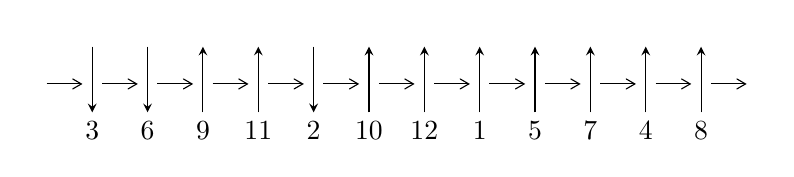
\begin{tikzpicture}[x=20pt, y=17pt]
	% nodes
	\node (C0) at (0, 0) {};
	\node (C1) at (1, 0) {};
	\node (C1U) at (1, +1) {};
	\node (C1D) at (1, -1) {3};

	\node (C2) at (2, 0) {};
	\node (C2U) at (2, +1) {};
	\node (C2D) at (2, -1) {6};

	\node (C3) at (3, 0) {};
	\node (C3U) at (3, +1) {};
	\node (C3D) at (3, -1) {9};

	\node (C4) at (4, 0) {};
	\node (C4U) at (4, +1) {};
	\node (C4D) at (4, -1) {11};

	\node (C5) at (5, 0) {};
	\node (C5U) at (5, +1) {};
	\node (C5D) at (5, -1) {2};

	\node (C6) at (6, 0) {};
	\node (C6U) at (6, +1) {};
	\node (C6D) at (6, -1) {10};

	\node (C7) at (7, 0) {};
	\node (C7U) at (7, +1) {};
	\node (C7D) at (7, -1) {12};

	\node (C8) at (8, 0) {};
	\node (C8U) at (8, +1) {};
	\node (C8D) at (8, -1) {1};

	\node (C9) at (9, 0) {};
	\node (C9U) at (9, +1) {};
	\node (C9D) at (9, -1) {5};

	\node (C10) at (10, 0) {};
	\node (C10U) at (10, +1) {};
	\node (C10D) at (10, -1) {7};

	\node (C11) at (11, 0) {};
	\node (C11U) at (11, +1) {};
	\node (C11D) at (11, -1) {4};

	\node (C12) at (12, 0) {};
	\node (C12U) at (12, +1) {};
	\node (C12D) at (12, -1) {8};
	\node (C13) at (13, 0) {};

	% arrows
	\draw[->,>={angle 60}]
	(C0) edge (C1) (C1) edge (C2) (C2) edge (C3) (C3) edge (C4) (C4) edge (C5) (C5) edge (C6) (C6) edge (C7) (C7) edge (C8) (C8) edge (C9) (C9) edge (C10) (C10) edge (C11) (C11) edge (C12) (C12) edge (C13) ;	\draw[->,>=stealth]
	(C1U) edge (C1D) (C2U) edge (C2D) (C3D) edge (C3U) (C4D) edge (C4U) (C5U) edge (C5D) (C6D) edge (C6U) (C7D) edge (C7U) (C8D) edge (C8U) (C9D) edge (C9U) (C10D) edge (C10U) (C11D) edge (C11U) (C12D) edge (C12U) ;
	\end{tikzpicture} \\
\hhline{~~} \\& 
\textbf{Solving Sequence} \\ \cline{2-2} 
 &
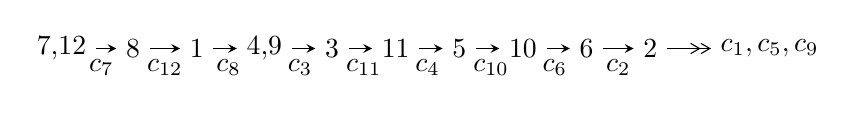
\begin{tikzpicture}[x=23pt, y=7pt]
	% node
	\node (A0) at (-1/8, 0) {7,12};
	\node (A1) at (1, 0) {8};
	\node (A2) at (2, 0) {1};
	\node (A3) at (49/16, 0) {4,9};
	\node (A4) at (33/8, 0) {3};
	\node (A5) at (41/8, 0) {11};
	\node (A6) at (49/8, 0) {5};
	\node (A7) at (57/8, 0) {10};
	\node (A8) at (65/8, 0) {6};
	\node (A9) at (73/8, 0) {2};
	\node (C1) at (1/2, -1) {$c_{7}$};
	\node (C2) at (3/2, -1) {$c_{12}$};
	\node (C3) at (5/2, -1) {$c_{8}$};
	\node (C4) at (29/8, -1) {$c_{3}$};
	\node (C5) at (37/8, -1) {$c_{11}$};
	\node (C6) at (45/8, -1) {$c_{4}$};
	\node (C7) at (53/8, -1) {$c_{10}$};
	\node (C8) at (61/8, -1) {$c_{6}$};
	\node (C9) at (69/8, -1) {$c_{2}$};
	\node (A10) at (11, 0) {$c_{1},c_{5},c_{9}$};

	% edge
	\draw[->,>=stealth]	
	(A0) edge (A1) (A1) edge (A2) (A2) edge (A3) (A3) edge (A4) (A4) edge (A5) (A5) edge (A6) (A6) edge (A7) (A7) edge (A8) (A8) edge (A9) ;
	\draw[->>,>={angle 60}]	
	(A9) edge (A10);
\end{tikzpicture} \\ 

\end{tabular} \\

\footnotetext{
The image of knot diagram is generated by the software ``\textbf{Draw programme}" developed by Andrew Bartholomew(\url{http://www.layer8.co.uk/maths/draw/index.htm\#Running-draw}), where we modified some parts for our purpose(\url{https://github.com/CATsTAILs/LinksPainter}).
}\phantom \\ \newline 
\centering \textbf{Ideals for irreducible components\footnotemark of $X_{\text{par}}$} 
 
\begin{align*}
I^u_{1}&=\langle 
-2.00278\times10^{313} u^{114}+8.20350\times10^{313} u^{113}+\cdots+2.57348\times10^{314} b+1.42070\times10^{315},\\
\phantom{I^u_{1}}&\phantom{= \langle  }8.24259\times10^{314} u^{114}-1.69226\times10^{315} u^{113}+\cdots+2.57348\times10^{314} a-9.87325\times10^{315},\\
\phantom{I^u_{1}}&\phantom{= \langle  }u^{115}-2 u^{114}+\cdots-28 u+1\rangle \\
I^u_{2}&=\langle 
u^{24}-14 u^{22}+\cdots+b+2,\;u^{24}+u^{23}+\cdots+a+u,\;u^{25}+u^{24}+\cdots+u+1\rangle \\
\\
\end{align*}
\raggedright * 2 irreducible components of $\dim_{\mathbb{C}}=0$, with total 140 representations.\\
\footnotetext{All coefficients of polynomials are rational numbers. But the coefficients are sometimes approximated in decimal forms when there is not enough margin.}
\newpage
\renewcommand{\arraystretch}{1}
\centering \section*{I. $I^u_{1}= \langle -2.00\times10^{313} u^{114}+8.20\times10^{313} u^{113}+\cdots+2.57\times10^{314} b+1.42\times10^{315},\;8.24\times10^{314} u^{114}-1.69\times10^{315} u^{113}+\cdots+2.57\times10^{314} a-9.87\times10^{315},\;u^{115}-2 u^{114}+\cdots-28 u+1 \rangle$}
\flushleft \textbf{(i) Arc colorings}\\
\begin{tabular}{m{7pt} m{180pt} m{7pt} m{180pt} }
\flushright $a_{7}=$&$\begin{pmatrix}1\\0\end{pmatrix}$ \\
\flushright $a_{12}=$&$\begin{pmatrix}0\\u\end{pmatrix}$ \\
\flushright $a_{8}=$&$\begin{pmatrix}1\\- u^2\end{pmatrix}$ \\
\flushright $a_{1}=$&$\begin{pmatrix}u\\- u^3+u\end{pmatrix}$ \\
\flushright $a_{4}=$&$\begin{pmatrix}-3.20290 u^{114}+6.57577 u^{113}+\cdots-705.319 u+38.3654\\0.0778241 u^{114}-0.318771 u^{113}+\cdots+56.3225 u-5.52054\end{pmatrix}$ \\
\flushright $a_{9}=$&$\begin{pmatrix}- u^2+1\\u^4-2 u^2\end{pmatrix}$ \\
\flushright $a_{3}=$&$\begin{pmatrix}-3.38717 u^{114}+7.04311 u^{113}+\cdots-764.082 u+43.7198\\0.0236815 u^{114}-0.267953 u^{113}+\cdots+53.7249 u-5.44079\end{pmatrix}$ \\
\flushright $a_{11}=$&$\begin{pmatrix}-3.85922 u^{114}+7.71029 u^{113}+\cdots-891.654 u+57.0291\\-0.559786 u^{114}+0.840056 u^{113}+\cdots-68.2350 u+2.71601\end{pmatrix}$ \\
\flushright $a_{5}=$&$\begin{pmatrix}-3.04090 u^{114}+4.84465 u^{113}+\cdots-648.834 u+44.1418\\0.0779924 u^{114}+0.105782 u^{113}+\cdots-11.6253 u-0.201228\end{pmatrix}$ \\
\flushright $a_{10}=$&$\begin{pmatrix}-3.29943 u^{114}+6.87024 u^{113}+\cdots-823.419 u+54.3131\\-0.559786 u^{114}+0.840056 u^{113}+\cdots-68.2350 u+2.71601\end{pmatrix}$ \\
\flushright $a_{6}=$&$\begin{pmatrix}2.09218 u^{114}-4.51224 u^{113}+\cdots+462.352 u-45.9770\\1.33271 u^{114}-2.35933 u^{113}+\cdots+187.582 u-9.48403\end{pmatrix}$ \\
\flushright $a_{2}=$&$\begin{pmatrix}-2.61490 u^{114}+4.63695 u^{113}+\cdots-629.293 u+45.1624\\-0.985977 u^{114}+1.87369 u^{113}+\cdots-139.022 u+6.55447\end{pmatrix}$\\&\end{tabular}
\flushleft \textbf{(ii) Obstruction class $= -1$}\\~\\
\flushleft \textbf{(iii) Cusp Shapes $= -3.86736 u^{114}+7.91239 u^{113}+\cdots-545.310 u+42.5006$}\\~\\
\newpage\renewcommand{\arraystretch}{1}
\flushleft \textbf{(iv) u-Polynomials at the component}\newline \\
\begin{tabular}{m{50pt}|m{274pt}}
Crossings & \hspace{64pt}u-Polynomials at each crossing \\
\hline $$\begin{aligned}c_{1}\end{aligned}$$&$\begin{aligned}
&u^{115}+42 u^{114}+\cdots+430 u+1
\end{aligned}$\\
\hline $$\begin{aligned}c_{2},c_{5}\end{aligned}$$&$\begin{aligned}
&u^{115}+6 u^{114}+\cdots+34 u+1
\end{aligned}$\\
\hline $$\begin{aligned}c_{3}\end{aligned}$$&$\begin{aligned}
&u^{115}- u^{114}+\cdots+382316 u-23801
\end{aligned}$\\
\hline $$\begin{aligned}c_{4},c_{11}\end{aligned}$$&$\begin{aligned}
&u^{115}-3 u^{114}+\cdots+2 u-1
\end{aligned}$\\
\hline $$\begin{aligned}c_{6},c_{10}\end{aligned}$$&$\begin{aligned}
&u^{115}+3 u^{114}+\cdots+416 u+649
\end{aligned}$\\
\hline $$\begin{aligned}c_{7},c_{8},c_{12}\end{aligned}$$&$\begin{aligned}
&u^{115}+2 u^{114}+\cdots-28 u-1
\end{aligned}$\\
\hline $$\begin{aligned}c_{9}\end{aligned}$$&$\begin{aligned}
&u^{115}+u^{114}+\cdots-1504 u-71
\end{aligned}$\\
\hline
\end{tabular}\\~\\
\newpage\renewcommand{\arraystretch}{1}
\flushleft \textbf{(v) Riley Polynomials at the component}\newline \\
\begin{tabular}{m{50pt}|m{274pt}}
Crossings & \hspace{64pt}Riley Polynomials at each crossing \\
\hline $$\begin{aligned}c_{1}\end{aligned}$$&$\begin{aligned}
&y^{115}+74 y^{114}+\cdots-137646 y-1
\end{aligned}$\\
\hline $$\begin{aligned}c_{2},c_{5}\end{aligned}$$&$\begin{aligned}
&y^{115}-42 y^{114}+\cdots+430 y-1
\end{aligned}$\\
\hline $$\begin{aligned}c_{3}\end{aligned}$$&$\begin{aligned}
&y^{115}-35 y^{114}+\cdots+165406395062 y-566487601
\end{aligned}$\\
\hline $$\begin{aligned}c_{4},c_{11}\end{aligned}$$&$\begin{aligned}
&y^{115}+65 y^{114}+\cdots-6 y-1
\end{aligned}$\\
\hline $$\begin{aligned}c_{6},c_{10}\end{aligned}$$&$\begin{aligned}
&y^{115}-91 y^{114}+\cdots+19697572 y-421201
\end{aligned}$\\
\hline $$\begin{aligned}c_{7},c_{8},c_{12}\end{aligned}$$&$\begin{aligned}
&y^{115}-120 y^{114}+\cdots+232 y-1
\end{aligned}$\\
\hline $$\begin{aligned}c_{9}\end{aligned}$$&$\begin{aligned}
&y^{115}-23 y^{114}+\cdots+3132476 y-5041
\end{aligned}$\\
\hline
\end{tabular}\\~\\
\newpage\flushleft \textbf{(vi) Complex Volumes and Cusp Shapes}
$$\begin{array}{c|c|c}  
\text{Solutions to }I^u_{1}& \I (\text{vol} + \sqrt{-1}CS) & \text{Cusp shape}\\
 \hline 
\begin{aligned}
u &= \phantom{-}1.018240 + 0.185716 I \\
a &= -0.157187 - 1.384820 I \\
b &= -0.224318 + 1.063560 I\end{aligned}
 & -4.54218 + 1.04428 I & \phantom{-0.000000 } 0 \\ \hline\begin{aligned}
u &= \phantom{-}1.018240 - 0.185716 I \\
a &= -0.157187 + 1.384820 I \\
b &= -0.224318 - 1.063560 I\end{aligned}
 & -4.54218 - 1.04428 I & \phantom{-0.000000 } 0 \\ \hline\begin{aligned}
u &= -0.605009 + 0.839926 I \\
a &= -1.257980 + 0.199905 I \\
b &= -1.54849 - 0.88534 I\end{aligned}
 & \phantom{-}2.94287 - 7.58492 I & \phantom{-0.000000 } 0 \\ \hline\begin{aligned}
u &= -0.605009 - 0.839926 I \\
a &= -1.257980 - 0.199905 I \\
b &= -1.54849 + 0.88534 I\end{aligned}
 & \phantom{-}2.94287 + 7.58492 I & \phantom{-0.000000 } 0 \\ \hline\begin{aligned}
u &= \phantom{-}0.110734 + 1.038700 I \\
a &= -0.804178 + 0.323589 I \\
b &= -1.62068 + 0.68689 I\end{aligned}
 & \phantom{-}3.09318 + 2.07281 I & \phantom{-0.000000 } 0 \\ \hline\begin{aligned}
u &= \phantom{-}0.110734 - 1.038700 I \\
a &= -0.804178 - 0.323589 I \\
b &= -1.62068 - 0.68689 I\end{aligned}
 & \phantom{-}3.09318 - 2.07281 I & \phantom{-0.000000 } 0 \\ \hline\begin{aligned}
u &= \phantom{-}0.275186 + 1.040870 I \\
a &= \phantom{-}0.794196 - 0.193683 I \\
b &= \phantom{-}1.62388 - 0.79412 I\end{aligned}
 & \phantom{-}2.42939 - 3.12525 I & \phantom{-0.000000 } 0 \\ \hline\begin{aligned}
u &= \phantom{-}0.275186 - 1.040870 I \\
a &= \phantom{-}0.794196 + 0.193683 I \\
b &= \phantom{-}1.62388 + 0.79412 I\end{aligned}
 & \phantom{-}2.42939 + 3.12525 I & \phantom{-0.000000 } 0 \\ \hline\begin{aligned}
u &= -0.585102 + 0.950055 I \\
a &= \phantom{-}1.170430 - 0.104503 I \\
b &= \phantom{-}1.67909 + 0.83613 I\end{aligned}
 & \phantom{-}1.56496 - 13.32550 I & \phantom{-0.000000 } 0 \\ \hline\begin{aligned}
u &= -0.585102 - 0.950055 I \\
a &= \phantom{-}1.170430 + 0.104503 I \\
b &= \phantom{-}1.67909 - 0.83613 I\end{aligned}
 & \phantom{-}1.56496 + 13.32550 I & \phantom{-0.000000 } 0\\
 \hline 
 \end{array}$$\newpage$$\begin{array}{c|c|c}  
\text{Solutions to }I^u_{1}& \I (\text{vol} + \sqrt{-1}CS) & \text{Cusp shape}\\
 \hline 
\begin{aligned}
u &= -0.875304 + 0.010082 I \\
a &= -0.482427 + 0.797072 I \\
b &= -0.208353 + 0.555462 I\end{aligned}
 & \phantom{-}2.28782 + 2.70515 I & \phantom{-0.000000 } 0 \\ \hline\begin{aligned}
u &= -0.875304 - 0.010082 I \\
a &= -0.482427 - 0.797072 I \\
b &= -0.208353 - 0.555462 I\end{aligned}
 & \phantom{-}2.28782 - 2.70515 I & \phantom{-0.000000 } 0 \\ \hline\begin{aligned}
u &= \phantom{-}0.678698 + 0.545869 I \\
a &= -0.636932 + 0.805126 I \\
b &= \phantom{-}0.612781 - 0.051539 I\end{aligned}
 & \phantom{-}4.36100 + 8.04330 I & \phantom{-0.000000 } 0 \\ \hline\begin{aligned}
u &= \phantom{-}0.678698 - 0.545869 I \\
a &= -0.636932 - 0.805126 I \\
b &= \phantom{-}0.612781 + 0.051539 I\end{aligned}
 & \phantom{-}4.36100 - 8.04330 I & \phantom{-0.000000 } 0 \\ \hline\begin{aligned}
u &= -0.305379 + 0.810200 I \\
a &= \phantom{-}1.47601 + 0.19019 I \\
b &= \phantom{-}1.43158 + 0.51265 I\end{aligned}
 & -3.63406 - 6.53388 I & \phantom{-0.000000 } 0 \\ \hline\begin{aligned}
u &= -0.305379 - 0.810200 I \\
a &= \phantom{-}1.47601 - 0.19019 I \\
b &= \phantom{-}1.43158 - 0.51265 I\end{aligned}
 & -3.63406 + 6.53388 I & \phantom{-0.000000 } 0 \\ \hline\begin{aligned}
u &= -0.929618 + 0.653649 I \\
a &= \phantom{-}0.204466 - 0.892515 I \\
b &= \phantom{-}0.963248 + 0.154542 I\end{aligned}
 & -1.85464 + 1.48845 I & \phantom{-0.000000 } 0 \\ \hline\begin{aligned}
u &= -0.929618 - 0.653649 I \\
a &= \phantom{-}0.204466 + 0.892515 I \\
b &= \phantom{-}0.963248 - 0.154542 I\end{aligned}
 & -1.85464 - 1.48845 I & \phantom{-0.000000 } 0 \\ \hline\begin{aligned}
u &= \phantom{-}0.652482 + 0.542736 I \\
a &= -0.745445 - 1.183410 I \\
b &= -0.868838 + 0.692560 I\end{aligned}
 & -2.35658 - 3.07713 I & \phantom{-0.000000 } 0 \\ \hline\begin{aligned}
u &= \phantom{-}0.652482 - 0.542736 I \\
a &= -0.745445 + 1.183410 I \\
b &= -0.868838 - 0.692560 I\end{aligned}
 & -2.35658 + 3.07713 I & \phantom{-0.000000 } 0\\
 \hline 
 \end{array}$$\newpage$$\begin{array}{c|c|c}  
\text{Solutions to }I^u_{1}& \I (\text{vol} + \sqrt{-1}CS) & \text{Cusp shape}\\
 \hline 
\begin{aligned}
u &= \phantom{-}0.488617 + 0.692095 I \\
a &= -1.313310 - 0.468315 I \\
b &= -1.60980 - 0.02547 I\end{aligned}
 & -2.80354 + 7.46099 I & \phantom{-0.000000 } 0 \\ \hline\begin{aligned}
u &= \phantom{-}0.488617 - 0.692095 I \\
a &= -1.313310 + 0.468315 I \\
b &= -1.60980 + 0.02547 I\end{aligned}
 & -2.80354 - 7.46099 I & \phantom{-0.000000 } 0 \\ \hline\begin{aligned}
u &= -0.636844 + 1.013560 I \\
a &= -0.439819 + 0.712756 I \\
b &= -1.46937 + 0.06518 I\end{aligned}
 & \phantom{-}2.75509 + 1.57727 I & \phantom{-0.000000 } 0 \\ \hline\begin{aligned}
u &= -0.636844 - 1.013560 I \\
a &= -0.439819 - 0.712756 I \\
b &= -1.46937 - 0.06518 I\end{aligned}
 & \phantom{-}2.75509 - 1.57727 I & \phantom{-0.000000 } 0 \\ \hline\begin{aligned}
u &= \phantom{-}0.697646 + 0.385481 I \\
a &= \phantom{-}0.897484 - 0.735922 I \\
b &= -0.577128 + 0.043803 I\end{aligned}
 & \phantom{-}5.81339 + 2.21028 I & \phantom{-0.000000 } 0 \\ \hline\begin{aligned}
u &= \phantom{-}0.697646 - 0.385481 I \\
a &= \phantom{-}0.897484 + 0.735922 I \\
b &= -0.577128 - 0.043803 I\end{aligned}
 & \phantom{-}5.81339 - 2.21028 I & \phantom{-0.000000 } 0 \\ \hline\begin{aligned}
u &= \phantom{-}0.516034 + 0.600339 I \\
a &= \phantom{-}1.27874 + 0.61859 I \\
b &= \phantom{-}1.49364 - 0.17840 I\end{aligned}
 & -1.59675 + 2.50323 I & \phantom{-0.000000 } 0 \\ \hline\begin{aligned}
u &= \phantom{-}0.516034 - 0.600339 I \\
a &= \phantom{-}1.27874 - 0.61859 I \\
b &= \phantom{-}1.49364 + 0.17840 I\end{aligned}
 & -1.59675 - 2.50323 I & \phantom{-0.000000 } 0 \\ \hline\begin{aligned}
u &= \phantom{-}1.271320 + 0.050169 I \\
a &= \phantom{-}0.411686 + 0.322353 I \\
b &= \phantom{-}1.73294 - 0.45796 I\end{aligned}
 & \phantom{-}1.070530 + 0.175208 I & \phantom{-0.000000 } 0 \\ \hline\begin{aligned}
u &= \phantom{-}1.271320 - 0.050169 I \\
a &= \phantom{-}0.411686 - 0.322353 I \\
b &= \phantom{-}1.73294 + 0.45796 I\end{aligned}
 & \phantom{-}1.070530 - 0.175208 I & \phantom{-0.000000 } 0\\
 \hline 
 \end{array}$$\newpage$$\begin{array}{c|c|c}  
\text{Solutions to }I^u_{1}& \I (\text{vol} + \sqrt{-1}CS) & \text{Cusp shape}\\
 \hline 
\begin{aligned}
u &= \phantom{-}0.498264 + 0.497941 I \\
a &= \phantom{-}1.016200 + 0.976841 I \\
b &= \phantom{-}1.017610 - 0.496622 I\end{aligned}
 & -1.66106 + 1.37436 I & \phantom{-0.000000 } 0 \\ \hline\begin{aligned}
u &= \phantom{-}0.498264 - 0.497941 I \\
a &= \phantom{-}1.016200 - 0.976841 I \\
b &= \phantom{-}1.017610 + 0.496622 I\end{aligned}
 & -1.66106 - 1.37436 I & \phantom{-0.000000 } 0 \\ \hline\begin{aligned}
u &= -0.789711 + 1.027930 I \\
a &= \phantom{-}0.351565 - 0.708003 I \\
b &= \phantom{-}1.45014 + 0.10270 I\end{aligned}
 & \phantom{-}1.92862 + 6.79274 I & \phantom{-0.000000 } 0 \\ \hline\begin{aligned}
u &= -0.789711 - 1.027930 I \\
a &= \phantom{-}0.351565 + 0.708003 I \\
b &= \phantom{-}1.45014 - 0.10270 I\end{aligned}
 & \phantom{-}1.92862 - 6.79274 I & \phantom{-0.000000 } 0 \\ \hline\begin{aligned}
u &= \phantom{-}1.29832\phantom{ +0.000000I} \\
a &= \phantom{-}1.04923\phantom{ +0.000000I} \\
b &= \phantom{-}1.40950\phantom{ +0.000000I}\end{aligned}
 & \phantom{-}1.43686\phantom{ +0.000000I} & \phantom{-0.000000 } 0 \\ \hline\begin{aligned}
u &= -0.323095 + 0.615709 I \\
a &= \phantom{-}0.461147 + 0.706059 I \\
b &= \phantom{-}0.419162 + 0.114693 I\end{aligned}
 & \phantom{-}0.61372 - 4.18682 I & \phantom{-0.000000 } 0 \\ \hline\begin{aligned}
u &= -0.323095 - 0.615709 I \\
a &= \phantom{-}0.461147 - 0.706059 I \\
b &= \phantom{-}0.419162 - 0.114693 I\end{aligned}
 & \phantom{-}0.61372 + 4.18682 I & \phantom{-0.000000 } 0 \\ \hline\begin{aligned}
u &= -0.508419 + 0.472877 I \\
a &= -0.503800 - 0.581500 I \\
b &= -0.332541 - 0.142272 I\end{aligned}
 & \phantom{-}1.291470 + 0.512565 I & \phantom{-0.000000 } 0 \\ \hline\begin{aligned}
u &= -0.508419 - 0.472877 I \\
a &= -0.503800 + 0.581500 I \\
b &= -0.332541 + 0.142272 I\end{aligned}
 & \phantom{-}1.291470 - 0.512565 I & \phantom{-0.000000 } 0 \\ \hline\begin{aligned}
u &= -0.691075 + 0.008162 I \\
a &= \phantom{-}0.503183 - 1.159190 I \\
b &= -0.202881 - 0.749571 I\end{aligned}
 & \phantom{-}2.81155 - 2.16819 I & \phantom{-0.000000 } 0\\
 \hline 
 \end{array}$$\newpage$$\begin{array}{c|c|c}  
\text{Solutions to }I^u_{1}& \I (\text{vol} + \sqrt{-1}CS) & \text{Cusp shape}\\
 \hline 
\begin{aligned}
u &= -0.691075 - 0.008162 I \\
a &= \phantom{-}0.503183 + 1.159190 I \\
b &= -0.202881 + 0.749571 I\end{aligned}
 & \phantom{-}2.81155 + 2.16819 I & \phantom{-0.000000 } 0 \\ \hline\begin{aligned}
u &= \phantom{-}0.404482 + 0.553410 I \\
a &= \phantom{-}1.232900 + 0.332174 I \\
b &= \phantom{-}1.39428 - 0.78774 I\end{aligned}
 & -1.21336 + 1.54147 I & \phantom{-0.000000 } 0 \\ \hline\begin{aligned}
u &= \phantom{-}0.404482 - 0.553410 I \\
a &= \phantom{-}1.232900 - 0.332174 I \\
b &= \phantom{-}1.39428 + 0.78774 I\end{aligned}
 & -1.21336 - 1.54147 I & \phantom{-0.000000 } 0 \\ \hline\begin{aligned}
u &= -1.330080 + 0.134554 I \\
a &= -0.182284 - 1.009940 I \\
b &= \phantom{-}0.024693 + 0.436211 I\end{aligned}
 & \phantom{-}3.17278 - 3.33556 I & \phantom{-0.000000 } 0 \\ \hline\begin{aligned}
u &= -1.330080 - 0.134554 I \\
a &= -0.182284 + 1.009940 I \\
b &= \phantom{-}0.024693 - 0.436211 I\end{aligned}
 & \phantom{-}3.17278 + 3.33556 I & \phantom{-0.000000 } 0 \\ \hline\begin{aligned}
u &= -1.319720 + 0.218573 I \\
a &= -0.533328 + 0.810389 I \\
b &= -1.27843 - 1.67952 I\end{aligned}
 & \phantom{-}4.59691 - 4.51548 I & \phantom{-0.000000 } 0 \\ \hline\begin{aligned}
u &= -1.319720 - 0.218573 I \\
a &= -0.533328 - 0.810389 I \\
b &= -1.27843 + 1.67952 I\end{aligned}
 & \phantom{-}4.59691 + 4.51548 I & \phantom{-0.000000 } 0 \\ \hline\begin{aligned}
u &= \phantom{-}0.328499 + 0.563619 I \\
a &= -1.78017 - 0.62506 I \\
b &= -1.129840 - 0.196835 I\end{aligned}
 & -6.26920 + 1.55197 I & \phantom{-0.000000 } 0 \\ \hline\begin{aligned}
u &= \phantom{-}0.328499 - 0.563619 I \\
a &= -1.78017 + 0.62506 I \\
b &= -1.129840 + 0.196835 I\end{aligned}
 & -6.26920 - 1.55197 I & \phantom{-0.000000 } 0 \\ \hline\begin{aligned}
u &= -1.352080 + 0.055142 I \\
a &= -0.660200 - 0.792131 I \\
b &= -0.406617 + 0.087523 I\end{aligned}
 & \phantom{-}2.93578 - 2.96211 I & \phantom{-0.000000 } 0\\
 \hline 
 \end{array}$$\newpage$$\begin{array}{c|c|c}  
\text{Solutions to }I^u_{1}& \I (\text{vol} + \sqrt{-1}CS) & \text{Cusp shape}\\
 \hline 
\begin{aligned}
u &= -1.352080 - 0.055142 I \\
a &= -0.660200 + 0.792131 I \\
b &= -0.406617 - 0.087523 I\end{aligned}
 & \phantom{-}2.93578 + 2.96211 I & \phantom{-0.000000 } 0 \\ \hline\begin{aligned}
u &= -0.285481 + 0.553910 I \\
a &= -0.94736 + 1.17382 I \\
b &= -1.190160 + 0.562522 I\end{aligned}
 & \phantom{-}1.30137 + 1.64548 I & \phantom{-}6.00000 + 1.95387 I \\ \hline\begin{aligned}
u &= -0.285481 - 0.553910 I \\
a &= -0.94736 - 1.17382 I \\
b &= -1.190160 - 0.562522 I\end{aligned}
 & \phantom{-}1.30137 - 1.64548 I & \phantom{-}6.00000 - 1.95387 I \\ \hline\begin{aligned}
u &= \phantom{-}1.377400 + 0.112468 I \\
a &= \phantom{-}0.235643 - 0.389792 I \\
b &= \phantom{-}1.75504 + 0.00095 I\end{aligned}
 & \phantom{-}5.67734 + 6.92704 I & \phantom{-0.000000 } 0 \\ \hline\begin{aligned}
u &= \phantom{-}1.377400 - 0.112468 I \\
a &= \phantom{-}0.235643 + 0.389792 I \\
b &= \phantom{-}1.75504 - 0.00095 I\end{aligned}
 & \phantom{-}5.67734 - 6.92704 I & \phantom{-0.000000 } 0 \\ \hline\begin{aligned}
u &= \phantom{-}1.41551 + 0.05574 I \\
a &= -0.249296 + 0.336866 I \\
b &= -1.54864 - 0.04612 I\end{aligned}
 & \phantom{-}7.15767 + 1.38994 I & \phantom{-0.000000 } 0 \\ \hline\begin{aligned}
u &= \phantom{-}1.41551 - 0.05574 I \\
a &= -0.249296 - 0.336866 I \\
b &= -1.54864 + 0.04612 I\end{aligned}
 & \phantom{-}7.15767 - 1.38994 I & \phantom{-0.000000 } 0 \\ \hline\begin{aligned}
u &= \phantom{-}1.42040 + 0.02638 I \\
a &= \phantom{-}0.12259 - 1.43678 I \\
b &= \phantom{-}0.094743 + 1.207000 I\end{aligned}
 & \phantom{-}4.01824 + 3.75134 I & \phantom{-0.000000 } 0 \\ \hline\begin{aligned}
u &= \phantom{-}1.42040 - 0.02638 I \\
a &= \phantom{-}0.12259 + 1.43678 I \\
b &= \phantom{-}0.094743 - 1.207000 I\end{aligned}
 & \phantom{-}4.01824 - 3.75134 I & \phantom{-0.000000 } 0 \\ \hline\begin{aligned}
u &= -1.43115 + 0.00636 I \\
a &= -0.342602 + 0.821484 I \\
b &= -1.48878 - 1.90769 I\end{aligned}
 & \phantom{-}7.97719 - 1.10739 I & \phantom{-0.000000 } 0\\
 \hline 
 \end{array}$$\newpage$$\begin{array}{c|c|c}  
\text{Solutions to }I^u_{1}& \I (\text{vol} + \sqrt{-1}CS) & \text{Cusp shape}\\
 \hline 
\begin{aligned}
u &= -1.43115 - 0.00636 I \\
a &= -0.342602 - 0.821484 I \\
b &= -1.48878 + 1.90769 I\end{aligned}
 & \phantom{-}7.97719 + 1.10739 I & \phantom{-0.000000 } 0 \\ \hline\begin{aligned}
u &= \phantom{-}1.42538 + 0.13458 I \\
a &= -0.887686 - 0.837109 I \\
b &= -1.14358 + 0.89620 I\end{aligned}
 & \phantom{-}7.13739 + 5.87227 I & \phantom{-0.000000 } 0 \\ \hline\begin{aligned}
u &= \phantom{-}1.42538 - 0.13458 I \\
a &= -0.887686 + 0.837109 I \\
b &= -1.14358 - 0.89620 I\end{aligned}
 & \phantom{-}7.13739 - 5.87227 I & \phantom{-0.000000 } 0 \\ \hline\begin{aligned}
u &= \phantom{-}1.39669 + 0.31721 I \\
a &= \phantom{-}0.364316 + 0.211138 I \\
b &= \phantom{-}1.28444 - 0.91618 I\end{aligned}
 & \phantom{-}5.83758 + 7.50527 I & \phantom{-0.000000 } 0 \\ \hline\begin{aligned}
u &= \phantom{-}1.39669 - 0.31721 I \\
a &= \phantom{-}0.364316 - 0.211138 I \\
b &= \phantom{-}1.28444 + 0.91618 I\end{aligned}
 & \phantom{-}5.83758 - 7.50527 I & \phantom{-0.000000 } 0 \\ \hline\begin{aligned}
u &= -1.42555 + 0.19539 I \\
a &= -0.471933 + 0.660900 I \\
b &= -1.39717 - 0.25537 I\end{aligned}
 & -0.61246 - 4.33479 I & \phantom{-0.000000 } 0 \\ \hline\begin{aligned}
u &= -1.42555 - 0.19539 I \\
a &= -0.471933 - 0.660900 I \\
b &= -1.39717 + 0.25537 I\end{aligned}
 & -0.61246 + 4.33479 I & \phantom{-0.000000 } 0 \\ \hline\begin{aligned}
u &= \phantom{-}1.42457 + 0.27958 I \\
a &= \phantom{-}0.734432 + 0.699953 I \\
b &= \phantom{-}1.51640 - 1.08330 I\end{aligned}
 & \phantom{-}1.88870 + 10.41200 I & \phantom{-0.000000 } 0 \\ \hline\begin{aligned}
u &= \phantom{-}1.42457 - 0.27958 I \\
a &= \phantom{-}0.734432 - 0.699953 I \\
b &= \phantom{-}1.51640 + 1.08330 I\end{aligned}
 & \phantom{-}1.88870 - 10.41200 I & \phantom{-0.000000 } 0 \\ \hline\begin{aligned}
u &= \phantom{-}1.43635 + 0.21406 I \\
a &= -0.341682 - 0.222471 I \\
b &= -1.25038 + 0.72200 I\end{aligned}
 & \phantom{-}7.27814 + 1.83894 I & \phantom{-0.000000 } 0\\
 \hline 
 \end{array}$$\newpage$$\begin{array}{c|c|c}  
\text{Solutions to }I^u_{1}& \I (\text{vol} + \sqrt{-1}CS) & \text{Cusp shape}\\
 \hline 
\begin{aligned}
u &= \phantom{-}1.43635 - 0.21406 I \\
a &= -0.341682 + 0.222471 I \\
b &= -1.25038 - 0.72200 I\end{aligned}
 & \phantom{-}7.27814 - 1.83894 I & \phantom{-0.000000 } 0 \\ \hline\begin{aligned}
u &= -1.47021 + 0.03880 I \\
a &= \phantom{-}0.431408 - 0.752415 I \\
b &= \phantom{-}0.751331 + 0.624823 I\end{aligned}
 & \phantom{-}4.94397 - 2.66854 I & \phantom{-0.000000 } 0 \\ \hline\begin{aligned}
u &= -1.47021 - 0.03880 I \\
a &= \phantom{-}0.431408 + 0.752415 I \\
b &= \phantom{-}0.751331 - 0.624823 I\end{aligned}
 & \phantom{-}4.94397 + 2.66854 I & \phantom{-0.000000 } 0 \\ \hline\begin{aligned}
u &= \phantom{-}1.47981\phantom{ +0.000000I} \\
a &= \phantom{-}0.430171\phantom{ +0.000000I} \\
b &= -0.102083\phantom{ +0.000000I}\end{aligned}
 & \phantom{-}7.68909\phantom{ +0.000000I} & \phantom{-0.000000 } 0 \\ \hline\begin{aligned}
u &= -0.284851 + 0.429526 I \\
a &= -2.70467 + 0.11196 I \\
b &= -0.916650 - 0.616764 I\end{aligned}
 & \phantom{-}1.60459 - 3.84172 I & \phantom{-}8.84200 + 10.85813 I \\ \hline\begin{aligned}
u &= -0.284851 - 0.429526 I \\
a &= -2.70467 - 0.11196 I \\
b &= -0.916650 + 0.616764 I\end{aligned}
 & \phantom{-}1.60459 + 3.84172 I & \phantom{-}8.84200 - 10.85813 I \\ \hline\begin{aligned}
u &= -1.48438 + 0.03284 I \\
a &= \phantom{-}0.343307 - 0.777614 I \\
b &= \phantom{-}1.60424 + 1.82962 I\end{aligned}
 & \phantom{-}8.16254 - 6.34416 I & \phantom{-0.000000 } 0 \\ \hline\begin{aligned}
u &= -1.48438 - 0.03284 I \\
a &= \phantom{-}0.343307 + 0.777614 I \\
b &= \phantom{-}1.60424 - 1.82962 I\end{aligned}
 & \phantom{-}8.16254 + 6.34416 I & \phantom{-0.000000 } 0 \\ \hline\begin{aligned}
u &= \phantom{-}0.218770 + 0.450408 I \\
a &= \phantom{-}0.73303 + 1.25721 I \\
b &= \phantom{-}0.697553 - 0.256568 I\end{aligned}
 & -1.60581 + 1.06805 I & -0.56189 - 2.30198 I \\ \hline\begin{aligned}
u &= \phantom{-}0.218770 - 0.450408 I \\
a &= \phantom{-}0.73303 - 1.25721 I \\
b &= \phantom{-}0.697553 + 0.256568 I\end{aligned}
 & -1.60581 - 1.06805 I & -0.56189 + 2.30198 I\\
 \hline 
 \end{array}$$\newpage$$\begin{array}{c|c|c}  
\text{Solutions to }I^u_{1}& \I (\text{vol} + \sqrt{-1}CS) & \text{Cusp shape}\\
 \hline 
\begin{aligned}
u &= \phantom{-}0.171797 + 0.464235 I \\
a &= \phantom{-}0.62471 + 1.85083 I \\
b &= \phantom{-}0.701346 - 0.001848 I\end{aligned}
 & -1.57573 + 1.11003 I & -1.82221 - 3.85918 I \\ \hline\begin{aligned}
u &= \phantom{-}0.171797 - 0.464235 I \\
a &= \phantom{-}0.62471 - 1.85083 I \\
b &= \phantom{-}0.701346 + 0.001848 I\end{aligned}
 & -1.57573 - 1.11003 I & -1.82221 + 3.85918 I \\ \hline\begin{aligned}
u &= -1.52617 + 0.17115 I \\
a &= \phantom{-}0.422183 - 0.701863 I \\
b &= \phantom{-}1.35404 + 1.44231 I\end{aligned}
 & \phantom{-}5.33523 - 4.21971 I & \phantom{-0.000000 } 0 \\ \hline\begin{aligned}
u &= -1.52617 - 0.17115 I \\
a &= \phantom{-}0.422183 + 0.701863 I \\
b &= \phantom{-}1.35404 - 1.44231 I\end{aligned}
 & \phantom{-}5.33523 + 4.21971 I & \phantom{-0.000000 } 0 \\ \hline\begin{aligned}
u &= -0.459350\phantom{ +0.000000I} \\
a &= -0.616527\phantom{ +0.000000I} \\
b &= -0.196835\phantom{ +0.000000I}\end{aligned}
 & \phantom{-}0.646841\phantom{ +0.000000I} & \phantom{-}15.6940\phantom{ +0.000000I} \\ \hline\begin{aligned}
u &= -1.52857 + 0.19712 I \\
a &= \phantom{-}0.416577 - 0.652874 I \\
b &= \phantom{-}1.73061 + 0.73350 I\end{aligned}
 & \phantom{-}5.16134 - 5.41994 I & \phantom{-0.000000 } 0 \\ \hline\begin{aligned}
u &= -1.52857 - 0.19712 I \\
a &= \phantom{-}0.416577 + 0.652874 I \\
b &= \phantom{-}1.73061 - 0.73350 I\end{aligned}
 & \phantom{-}5.16134 + 5.41994 I & \phantom{-0.000000 } 0 \\ \hline\begin{aligned}
u &= -1.54013 + 0.13822 I \\
a &= \phantom{-}0.901321 + 0.306423 I \\
b &= \phantom{-}0.153566 + 0.050367 I\end{aligned}
 & \phantom{-}13.13020 - 4.23147 I & \phantom{-0.000000 } 0 \\ \hline\begin{aligned}
u &= -1.54013 - 0.13822 I \\
a &= \phantom{-}0.901321 - 0.306423 I \\
b &= \phantom{-}0.153566 - 0.050367 I\end{aligned}
 & \phantom{-}13.13020 + 4.23147 I & \phantom{-0.000000 } 0 \\ \hline\begin{aligned}
u &= -1.52843 + 0.23524 I \\
a &= -0.421757 + 0.632040 I \\
b &= -1.89537 - 0.56177 I\end{aligned}
 & \phantom{-}3.83848 - 10.84980 I & \phantom{-0.000000 } 0\\
 \hline 
 \end{array}$$\newpage$$\begin{array}{c|c|c}  
\text{Solutions to }I^u_{1}& \I (\text{vol} + \sqrt{-1}CS) & \text{Cusp shape}\\
 \hline 
\begin{aligned}
u &= -1.52843 - 0.23524 I \\
a &= -0.421757 - 0.632040 I \\
b &= -1.89537 + 0.56177 I\end{aligned}
 & \phantom{-}3.83848 + 10.84980 I & \phantom{-0.000000 } 0 \\ \hline\begin{aligned}
u &= -1.55259 + 0.18914 I \\
a &= -0.816437 - 0.313853 I \\
b &= -0.151088 - 0.077565 I\end{aligned}
 & \phantom{-}11.6728 - 10.8282 I & \phantom{-0.000000 } 0 \\ \hline\begin{aligned}
u &= -1.55259 - 0.18914 I \\
a &= -0.816437 + 0.313853 I \\
b &= -0.151088 + 0.077565 I\end{aligned}
 & \phantom{-}11.6728 + 10.8282 I & \phantom{-0.000000 } 0 \\ \hline\begin{aligned}
u &= \phantom{-}1.56319 + 0.28705 I \\
a &= -0.630557 - 0.732829 I \\
b &= -1.45401 + 1.40123 I\end{aligned}
 & \phantom{-}10.0027 + 11.7199 I & \phantom{-0.000000 } 0 \\ \hline\begin{aligned}
u &= \phantom{-}1.56319 - 0.28705 I \\
a &= -0.630557 + 0.732829 I \\
b &= -1.45401 - 1.40123 I\end{aligned}
 & \phantom{-}10.0027 - 11.7199 I & \phantom{-0.000000 } 0 \\ \hline\begin{aligned}
u &= -1.53087 + 0.44466 I \\
a &= -0.538677 + 0.605984 I \\
b &= -1.27237 - 1.73794 I\end{aligned}
 & \phantom{-}8.51430 - 7.66393 I & \phantom{-0.000000 } 0 \\ \hline\begin{aligned}
u &= -1.53087 - 0.44466 I \\
a &= -0.538677 - 0.605984 I \\
b &= -1.27237 + 1.73794 I\end{aligned}
 & \phantom{-}8.51430 + 7.66393 I & \phantom{-0.000000 } 0 \\ \hline\begin{aligned}
u &= \phantom{-}1.60635 + 0.00240 I \\
a &= -0.194839 + 0.106575 I \\
b &= -0.461684 + 0.006920 I\end{aligned}
 & \phantom{-}7.99022 - 0.01147 I & \phantom{-0.000000 } 0 \\ \hline\begin{aligned}
u &= \phantom{-}1.60635 - 0.00240 I \\
a &= -0.194839 - 0.106575 I \\
b &= -0.461684 - 0.006920 I\end{aligned}
 & \phantom{-}7.99022 + 0.01147 I & \phantom{-0.000000 } 0 \\ \hline\begin{aligned}
u &= \phantom{-}1.57491 + 0.32730 I \\
a &= \phantom{-}0.620503 + 0.703580 I \\
b &= \phantom{-}1.54320 - 1.43840 I\end{aligned}
 & \phantom{-}8.5741 + 17.9836 I & \phantom{-0.000000 } 0\\
 \hline 
 \end{array}$$\newpage$$\begin{array}{c|c|c}  
\text{Solutions to }I^u_{1}& \I (\text{vol} + \sqrt{-1}CS) & \text{Cusp shape}\\
 \hline 
\begin{aligned}
u &= \phantom{-}1.57491 - 0.32730 I \\
a &= \phantom{-}0.620503 - 0.703580 I \\
b &= \phantom{-}1.54320 + 1.43840 I\end{aligned}
 & \phantom{-}8.5741 - 17.9836 I & \phantom{-0.000000 } 0 \\ \hline\begin{aligned}
u &= -1.59105 + 0.38347 I \\
a &= \phantom{-}0.495046 - 0.610111 I \\
b &= \phantom{-}1.19813 + 1.73205 I\end{aligned}
 & \phantom{-}8.66822 - 2.28109 I & \phantom{-0.000000 } 0 \\ \hline\begin{aligned}
u &= -1.59105 - 0.38347 I \\
a &= \phantom{-}0.495046 + 0.610111 I \\
b &= \phantom{-}1.19813 - 1.73205 I\end{aligned}
 & \phantom{-}8.66822 + 2.28109 I & \phantom{-0.000000 } 0 \\ \hline\begin{aligned}
u &= \phantom{-}1.65004 + 0.15658 I \\
a &= \phantom{-}0.362370 - 0.138439 I \\
b &= -0.032142 + 0.428821 I\end{aligned}
 & \phantom{-}11.24740 + 2.95138 I & \phantom{-0.000000 } 0 \\ \hline\begin{aligned}
u &= \phantom{-}1.65004 - 0.15658 I \\
a &= \phantom{-}0.362370 + 0.138439 I \\
b &= -0.032142 - 0.428821 I\end{aligned}
 & \phantom{-}11.24740 - 2.95138 I & \phantom{-0.000000 } 0 \\ \hline\begin{aligned}
u &= \phantom{-}1.65934 + 0.01198 I \\
a &= -0.016372 + 0.209351 I \\
b &= -0.132580 + 0.856158 I\end{aligned}
 & \phantom{-}11.19400 + 2.62330 I & \phantom{-0.000000 } 0 \\ \hline\begin{aligned}
u &= \phantom{-}1.65934 - 0.01198 I \\
a &= -0.016372 - 0.209351 I \\
b &= -0.132580 - 0.856158 I\end{aligned}
 & \phantom{-}11.19400 - 2.62330 I & \phantom{-0.000000 } 0 \\ \hline\begin{aligned}
u &= \phantom{-}1.68849 + 0.10230 I \\
a &= -0.339496 + 0.135960 I \\
b &= -0.087733 - 0.475697 I\end{aligned}
 & \phantom{-}11.33020 - 2.37820 I & \phantom{-0.000000 } 0 \\ \hline\begin{aligned}
u &= \phantom{-}1.68849 - 0.10230 I \\
a &= -0.339496 - 0.135960 I \\
b &= -0.087733 + 0.475697 I\end{aligned}
 & \phantom{-}11.33020 + 2.37820 I & \phantom{-0.000000 } 0 \\ \hline\begin{aligned}
u &= \phantom{-}0.265823 + 0.008631 I \\
a &= \phantom{-}1.48171 + 3.11119 I \\
b &= \phantom{-}1.51242 - 1.11418 I\end{aligned}
 & \phantom{-}2.11539 + 6.04579 I & \phantom{-}10.4529 - 10.3544 I\\
 \hline 
 \end{array}$$\newpage$$\begin{array}{c|c|c}  
\text{Solutions to }I^u_{1}& \I (\text{vol} + \sqrt{-1}CS) & \text{Cusp shape}\\
 \hline 
\begin{aligned}
u &= \phantom{-}0.265823 - 0.008631 I \\
a &= \phantom{-}1.48171 - 3.11119 I \\
b &= \phantom{-}1.51242 + 1.11418 I\end{aligned}
 & \phantom{-}2.11539 - 6.04579 I & \phantom{-}10.4529 + 10.3544 I \\ \hline\begin{aligned}
u &= -0.0385713 + 0.1129770 I \\
a &= -12.06090 + 6.19371 I \\
b &= -0.090997 - 0.588756 I\end{aligned}
 & -1.02861 - 3.32635 I & -5.1015 + 16.5830 I \\ \hline\begin{aligned}
u &= -0.0385713 - 0.1129770 I \\
a &= -12.06090 - 6.19371 I \\
b &= -0.090997 + 0.588756 I\end{aligned}
 & -1.02861 + 3.32635 I & -5.1015 - 16.5830 I \\ \hline\begin{aligned}
u &= \phantom{-}0.0748363 + 0.0173615 I \\
a &= -7.05729 - 9.61172 I \\
b &= -1.30476 + 1.14378 I\end{aligned}
 & \phantom{-}2.76607 + 1.01915 I & \phantom{-}12.89262 - 4.58125 I \\ \hline\begin{aligned}
u &= \phantom{-}0.0748363 - 0.0173615 I \\
a &= -7.05729 + 9.61172 I \\
b &= -1.30476 - 1.14378 I\end{aligned}
 & \phantom{-}2.76607 - 1.01915 I & \phantom{-}12.89262 + 4.58125 I\\
 \hline 
 \end{array}$$\newpage\newpage\renewcommand{\arraystretch}{1}
\centering \section*{II. $I^u_{2}= \langle u^{24}-14 u^{22}+\cdots+b+2,\;u^{24}+u^{23}+\cdots+a+u,\;u^{25}+u^{24}+\cdots+u+1 \rangle$}
\flushleft \textbf{(i) Arc colorings}\\
\begin{tabular}{m{7pt} m{180pt} m{7pt} m{180pt} }
\flushright $a_{7}=$&$\begin{pmatrix}1\\0\end{pmatrix}$ \\
\flushright $a_{12}=$&$\begin{pmatrix}0\\u\end{pmatrix}$ \\
\flushright $a_{8}=$&$\begin{pmatrix}1\\- u^2\end{pmatrix}$ \\
\flushright $a_{1}=$&$\begin{pmatrix}u\\- u^3+u\end{pmatrix}$ \\
\flushright $a_{4}=$&$\begin{pmatrix}- u^{24}- u^{23}+\cdots-3 u^2- u\\- u^{24}+14 u^{22}+\cdots- u-2\end{pmatrix}$ \\
\flushright $a_{9}=$&$\begin{pmatrix}- u^2+1\\u^4-2 u^2\end{pmatrix}$ \\
\flushright $a_{3}=$&$\begin{pmatrix}- u^{23}- u^{22}+\cdots- u+1\\- u^{24}+14 u^{22}+\cdots+8 u^2-2\end{pmatrix}$ \\
\flushright $a_{11}=$&$\begin{pmatrix}- u^{23}+14 u^{21}+\cdots+8 u+2\\u^2-1\end{pmatrix}$ \\
\flushright $a_{5}=$&$\begin{pmatrix}u^{23}+u^{22}+\cdots+8 u^2+u\\-2 u^{24}+28 u^{22}+\cdots- u-2\end{pmatrix}$ \\
\flushright $a_{10}=$&$\begin{pmatrix}- u^{23}+14 u^{21}+\cdots+8 u+3\\u^2-1\end{pmatrix}$ \\
\flushright $a_{6}=$&$\begin{pmatrix}u^{24}+u^{23}+\cdots-7 u-1\\u^4-2 u^2+1\end{pmatrix}$ \\
\flushright $a_{2}=$&$\begin{pmatrix}- u^{24}- u^{23}+\cdots+7 u+2\\- u^{24}+14 u^{22}+\cdots+4 u^2-2\end{pmatrix}$\\&\end{tabular}
\flushleft \textbf{(ii) Obstruction class $= 1$}\\~\\
\flushleft \textbf{(iii) Cusp Shapes $= 2 u^{24}-3 u^{23}-27 u^{22}+34 u^{21}+163 u^{20}-154 u^{19}-572 u^{18}+325 u^{17}+1266 u^{16}-185 u^{15}-1790 u^{14}-561 u^{13}+1547 u^{12}+1312 u^{11}-660 u^{10}-1220 u^9-117 u^8+571 u^7+326 u^6-108 u^5-144 u^4-31 u^3+15 u^2+11 u+9$}\\~\\
\newpage\renewcommand{\arraystretch}{1}
\flushleft \textbf{(iv) u-Polynomials at the component}\newline \\
\begin{tabular}{m{50pt}|m{274pt}}
Crossings & \hspace{64pt}u-Polynomials at each crossing \\
\hline $$\begin{aligned}c_{1}\end{aligned}$$&$\begin{aligned}
&u^{25}-11 u^{24}+\cdots+11 u-1
\end{aligned}$\\
\hline $$\begin{aligned}c_{2}\end{aligned}$$&$\begin{aligned}
&u^{25}- u^{24}+\cdots+u-1
\end{aligned}$\\
\hline $$\begin{aligned}c_{3}\end{aligned}$$&$\begin{aligned}
&u^{25}-2 u^{23}+\cdots- u+1
\end{aligned}$\\
\hline $$\begin{aligned}c_{4}\end{aligned}$$&$\begin{aligned}
&u^{25}+12 u^{23}+\cdots-3 u-1
\end{aligned}$\\
\hline $$\begin{aligned}c_{5}\end{aligned}$$&$\begin{aligned}
&u^{25}+u^{24}+\cdots+u+1
\end{aligned}$\\
\hline $$\begin{aligned}c_{6}\end{aligned}$$&$\begin{aligned}
&u^{25}-4 u^{24}+\cdots-7 u-3
\end{aligned}$\\
\hline $$\begin{aligned}c_{7},c_{8}\end{aligned}$$&$\begin{aligned}
&u^{25}+u^{24}+\cdots+u+1
\end{aligned}$\\
\hline $$\begin{aligned}c_{9}\end{aligned}$$&$\begin{aligned}
&u^{25}-2 u^{23}+\cdots-3 u-1
\end{aligned}$\\
\hline $$\begin{aligned}c_{10}\end{aligned}$$&$\begin{aligned}
&u^{25}+4 u^{24}+\cdots-7 u+3
\end{aligned}$\\
\hline $$\begin{aligned}c_{11}\end{aligned}$$&$\begin{aligned}
&u^{25}+12 u^{23}+\cdots-3 u+1
\end{aligned}$\\
\hline $$\begin{aligned}c_{12}\end{aligned}$$&$\begin{aligned}
&u^{25}- u^{24}+\cdots+u-1
\end{aligned}$\\
\hline
\end{tabular}\\~\\
\newpage\renewcommand{\arraystretch}{1}
\flushleft \textbf{(v) Riley Polynomials at the component}\newline \\
\begin{tabular}{m{50pt}|m{274pt}}
Crossings & \hspace{64pt}Riley Polynomials at each crossing \\
\hline $$\begin{aligned}c_{1}\end{aligned}$$&$\begin{aligned}
&y^{25}+17 y^{24}+\cdots-9 y-1
\end{aligned}$\\
\hline $$\begin{aligned}c_{2},c_{5}\end{aligned}$$&$\begin{aligned}
&y^{25}-11 y^{24}+\cdots+11 y-1
\end{aligned}$\\
\hline $$\begin{aligned}c_{3}\end{aligned}$$&$\begin{aligned}
&y^{25}-4 y^{24}+\cdots+7 y-1
\end{aligned}$\\
\hline $$\begin{aligned}c_{4},c_{11}\end{aligned}$$&$\begin{aligned}
&y^{25}+24 y^{24}+\cdots-21 y-1
\end{aligned}$\\
\hline $$\begin{aligned}c_{6},c_{10}\end{aligned}$$&$\begin{aligned}
&y^{25}-28 y^{24}+\cdots+109 y-9
\end{aligned}$\\
\hline $$\begin{aligned}c_{7},c_{8},c_{12}\end{aligned}$$&$\begin{aligned}
&y^{25}-29 y^{24}+\cdots+9 y-1
\end{aligned}$\\
\hline $$\begin{aligned}c_{9}\end{aligned}$$&$\begin{aligned}
&y^{25}-4 y^{24}+\cdots+5 y-1
\end{aligned}$\\
\hline
\end{tabular}\\~\\
\newpage\flushleft \textbf{(vi) Complex Volumes and Cusp Shapes}
$$\begin{array}{c|c|c}  
\text{Solutions to }I^u_{2}& \I (\text{vol} + \sqrt{-1}CS) & \text{Cusp shape}\\
 \hline 
\begin{aligned}
u &= \phantom{-}0.899524 + 0.143935 I \\
a &= -0.22000 - 1.49116 I \\
b &= \phantom{-}0.093617 + 0.808110 I\end{aligned}
 & -4.77060 + 0.53467 I & \phantom{-}1.18210 + 3.54286 I \\ \hline\begin{aligned}
u &= \phantom{-}0.899524 - 0.143935 I \\
a &= -0.22000 + 1.49116 I \\
b &= \phantom{-}0.093617 - 0.808110 I\end{aligned}
 & -4.77060 - 0.53467 I & \phantom{-}1.18210 - 3.54286 I \\ \hline\begin{aligned}
u &= -0.461491 + 0.651874 I \\
a &= -0.650192 + 0.796845 I \\
b &= -1.71465 + 0.47286 I\end{aligned}
 & \phantom{-}1.61103 + 5.13748 I & \phantom{-}5.49787 - 3.27489 I \\ \hline\begin{aligned}
u &= -0.461491 - 0.651874 I \\
a &= -0.650192 - 0.796845 I \\
b &= -1.71465 - 0.47286 I\end{aligned}
 & \phantom{-}1.61103 - 5.13748 I & \phantom{-}5.49787 + 3.27489 I \\ \hline\begin{aligned}
u &= -0.345068 + 0.672227 I \\
a &= \phantom{-}0.843939 - 0.815283 I \\
b &= \phantom{-}1.54914 - 0.69507 I\end{aligned}
 & \phantom{-}2.25062 + 0.31902 I & \phantom{-}6.04160 + 3.85521 I \\ \hline\begin{aligned}
u &= -0.345068 - 0.672227 I \\
a &= \phantom{-}0.843939 + 0.815283 I \\
b &= \phantom{-}1.54914 + 0.69507 I\end{aligned}
 & \phantom{-}2.25062 - 0.31902 I & \phantom{-}6.04160 - 3.85521 I \\ \hline\begin{aligned}
u &= -1.29243\phantom{ +0.000000I} \\
a &= -0.898087\phantom{ +0.000000I} \\
b &= -1.69102\phantom{ +0.000000I}\end{aligned}
 & \phantom{-}1.68877\phantom{ +0.000000I} & \phantom{-}24.9680\phantom{ +0.000000I} \\ \hline\begin{aligned}
u &= \phantom{-}1.336760 + 0.062255 I \\
a &= \phantom{-}0.25063 - 1.39537 I \\
b &= \phantom{-}0.118444 + 0.272340 I\end{aligned}
 & \phantom{-}2.76548 + 3.95750 I & \phantom{-}1.26642 - 10.15772 I \\ \hline\begin{aligned}
u &= \phantom{-}1.336760 - 0.062255 I \\
a &= \phantom{-}0.25063 + 1.39537 I \\
b &= \phantom{-}0.118444 - 0.272340 I\end{aligned}
 & \phantom{-}2.76548 - 3.95750 I & \phantom{-}1.26642 + 10.15772 I \\ \hline\begin{aligned}
u &= -0.604763 + 0.232407 I \\
a &= \phantom{-}0.094492 + 0.709624 I \\
b &= -1.058210 - 0.372015 I\end{aligned}
 & -0.894995 - 0.310970 I & \phantom{-}4.26361 - 1.77333 I\\
 \hline 
 \end{array}$$\newpage$$\begin{array}{c|c|c}  
\text{Solutions to }I^u_{2}& \I (\text{vol} + \sqrt{-1}CS) & \text{Cusp shape}\\
 \hline 
\begin{aligned}
u &= -0.604763 - 0.232407 I \\
a &= \phantom{-}0.094492 - 0.709624 I \\
b &= -1.058210 + 0.372015 I\end{aligned}
 & -0.894995 + 0.310970 I & \phantom{-}4.26361 + 1.77333 I \\ \hline\begin{aligned}
u &= -1.365210 + 0.285994 I \\
a &= -0.440687 + 0.557939 I \\
b &= -1.92813 - 1.45861 I\end{aligned}
 & \phantom{-}5.02864 - 8.59211 I & \phantom{-}8.28724 + 9.01089 I \\ \hline\begin{aligned}
u &= -1.365210 - 0.285994 I \\
a &= -0.440687 - 0.557939 I \\
b &= -1.92813 + 1.45861 I\end{aligned}
 & \phantom{-}5.02864 + 8.59211 I & \phantom{-}8.28724 - 9.01089 I \\ \hline\begin{aligned}
u &= -1.44588 + 0.24349 I \\
a &= \phantom{-}0.427346 - 0.651047 I \\
b &= \phantom{-}1.63249 + 1.65225 I\end{aligned}
 & \phantom{-}6.46764 - 3.71317 I & \phantom{-}11.06101 + 1.99584 I \\ \hline\begin{aligned}
u &= -1.44588 - 0.24349 I \\
a &= \phantom{-}0.427346 + 0.651047 I \\
b &= \phantom{-}1.63249 - 1.65225 I\end{aligned}
 & \phantom{-}6.46764 + 3.71317 I & \phantom{-}11.06101 - 1.99584 I \\ \hline\begin{aligned}
u &= -1.46192 + 0.13002 I \\
a &= \phantom{-}0.506435 - 0.863405 I \\
b &= \phantom{-}1.06541 + 1.44046 I\end{aligned}
 & \phantom{-}6.56506 - 4.68100 I & \phantom{-}11.18703 + 4.24370 I \\ \hline\begin{aligned}
u &= -1.46192 - 0.13002 I \\
a &= \phantom{-}0.506435 + 0.863405 I \\
b &= \phantom{-}1.06541 - 1.44046 I\end{aligned}
 & \phantom{-}6.56506 + 4.68100 I & \phantom{-}11.18703 - 4.24370 I \\ \hline\begin{aligned}
u &= -0.117385 + 0.504417 I \\
a &= \phantom{-}1.63922 - 1.22564 I \\
b &= \phantom{-}0.963769 - 0.734389 I\end{aligned}
 & \phantom{-}1.42552 + 2.47811 I & \phantom{-}5.45262 - 6.08221 I \\ \hline\begin{aligned}
u &= -0.117385 - 0.504417 I \\
a &= \phantom{-}1.63922 + 1.22564 I \\
b &= \phantom{-}0.963769 + 0.734389 I\end{aligned}
 & \phantom{-}1.42552 - 2.47811 I & \phantom{-}5.45262 + 6.08221 I \\ \hline\begin{aligned}
u &= \phantom{-}0.392045 + 0.179102 I \\
a &= -1.72754 - 2.97371 I \\
b &= -0.109614 + 0.850417 I\end{aligned}
 & -0.81902 - 3.09615 I & \phantom{-}13.37035 - 2.81210 I\\
 \hline 
 \end{array}$$\newpage$$\begin{array}{c|c|c}  
\text{Solutions to }I^u_{2}& \I (\text{vol} + \sqrt{-1}CS) & \text{Cusp shape}\\
 \hline 
\begin{aligned}
u &= \phantom{-}0.392045 - 0.179102 I \\
a &= -1.72754 + 2.97371 I \\
b &= -0.109614 - 0.850417 I\end{aligned}
 & -0.81902 + 3.09615 I & \phantom{-}13.37035 + 2.81210 I \\ \hline\begin{aligned}
u &= \phantom{-}1.60164 + 0.06657 I \\
a &= -0.254836 + 0.308818 I \\
b &= -0.212542 + 0.105314 I\end{aligned}
 & \phantom{-}8.22124 - 0.33216 I & \phantom{-}14.7793 + 12.1565 I \\ \hline\begin{aligned}
u &= \phantom{-}1.60164 - 0.06657 I \\
a &= -0.254836 - 0.308818 I \\
b &= -0.212542 - 0.105314 I\end{aligned}
 & \phantom{-}8.22124 + 0.33216 I & \phantom{-}14.7793 - 12.1565 I \\ \hline\begin{aligned}
u &= \phantom{-}1.71797 + 0.02033 I \\
a &= -0.019762 + 0.365389 I \\
b &= -0.054207 + 0.375046 I\end{aligned}
 & \phantom{-}10.78340 + 2.55543 I & \phantom{-0.000000 }      -6
0. 10   - 1.178635 I \\ \hline\begin{aligned}
u &= \phantom{-}1.71797 - 0.02033 I \\
a &= -0.019762 - 0.365389 I \\
b &= -0.054207 - 0.375046 I\end{aligned}
 & \phantom{-}10.78340 - 2.55543 I & \phantom{-0.000000 -}     -6
0. 10   + 1.178635 I\\
 \hline 
 \end{array}$$\newpage
\newpage\renewcommand{\arraystretch}{1}
\centering \section*{ III. u-Polynomials}
\begin{tabular}{m{50pt}|m{274pt}}
Crossings & \hspace{64pt}u-Polynomials at each crossing \\
\hline $$\begin{aligned}c_{1}\end{aligned}$$&$\begin{aligned}
&(u^{25}-11 u^{24}+\cdots+11 u-1)(u^{115}+42 u^{114}+\cdots+430 u+1)
\end{aligned}$\\
\hline $$\begin{aligned}c_{2}\end{aligned}$$&$\begin{aligned}
&(u^{25}- u^{24}+\cdots+u-1)(u^{115}+6 u^{114}+\cdots+34 u+1)
\end{aligned}$\\
\hline $$\begin{aligned}c_{3}\end{aligned}$$&$\begin{aligned}
&(u^{25}-2 u^{23}+\cdots- u+1)(u^{115}- u^{114}+\cdots+382316 u-23801)
\end{aligned}$\\
\hline $$\begin{aligned}c_{4}\end{aligned}$$&$\begin{aligned}
&(u^{25}+12 u^{23}+\cdots-3 u-1)(u^{115}-3 u^{114}+\cdots+2 u-1)
\end{aligned}$\\
\hline $$\begin{aligned}c_{5}\end{aligned}$$&$\begin{aligned}
&(u^{25}+u^{24}+\cdots+u+1)(u^{115}+6 u^{114}+\cdots+34 u+1)
\end{aligned}$\\
\hline $$\begin{aligned}c_{6}\end{aligned}$$&$\begin{aligned}
&(u^{25}-4 u^{24}+\cdots-7 u-3)(u^{115}+3 u^{114}+\cdots+416 u+649)
\end{aligned}$\\
\hline $$\begin{aligned}c_{7},c_{8}\end{aligned}$$&$\begin{aligned}
&(u^{25}+u^{24}+\cdots+u+1)(u^{115}+2 u^{114}+\cdots-28 u-1)
\end{aligned}$\\
\hline $$\begin{aligned}c_{9}\end{aligned}$$&$\begin{aligned}
&(u^{25}-2 u^{23}+\cdots-3 u-1)(u^{115}+u^{114}+\cdots-1504 u-71)
\end{aligned}$\\
\hline $$\begin{aligned}c_{10}\end{aligned}$$&$\begin{aligned}
&(u^{25}+4 u^{24}+\cdots-7 u+3)(u^{115}+3 u^{114}+\cdots+416 u+649)
\end{aligned}$\\
\hline $$\begin{aligned}c_{11}\end{aligned}$$&$\begin{aligned}
&(u^{25}+12 u^{23}+\cdots-3 u+1)(u^{115}-3 u^{114}+\cdots+2 u-1)
\end{aligned}$\\
\hline $$\begin{aligned}c_{12}\end{aligned}$$&$\begin{aligned}
&(u^{25}- u^{24}+\cdots+u-1)(u^{115}+2 u^{114}+\cdots-28 u-1)
\end{aligned}$\\
\hline
\end{tabular}\newpage\renewcommand{\arraystretch}{1}
\centering \section*{ IV. Riley Polynomials}
\begin{tabular}{m{50pt}|m{274pt}}
Crossings & \hspace{64pt}Riley Polynomials at each crossing \\
\hline $$\begin{aligned}c_{1}\end{aligned}$$&$\begin{aligned}
&(y^{25}+17 y^{24}+\cdots-9 y-1)(y^{115}+74 y^{114}+\cdots-137646 y-1)
\end{aligned}$\\
\hline $$\begin{aligned}c_{2},c_{5}\end{aligned}$$&$\begin{aligned}
&(y^{25}-11 y^{24}+\cdots+11 y-1)(y^{115}-42 y^{114}+\cdots+430 y-1)
\end{aligned}$\\
\hline $$\begin{aligned}c_{3}\end{aligned}$$&$\begin{aligned}
&(y^{25}-4 y^{24}+\cdots+7 y-1)\\
&\cdot(y^{115}-35 y^{114}+\cdots+165406395062 y-566487601)
\end{aligned}$\\
\hline $$\begin{aligned}c_{4},c_{11}\end{aligned}$$&$\begin{aligned}
&(y^{25}+24 y^{24}+\cdots-21 y-1)(y^{115}+65 y^{114}+\cdots-6 y-1)
\end{aligned}$\\
\hline $$\begin{aligned}c_{6},c_{10}\end{aligned}$$&$\begin{aligned}
&(y^{25}-28 y^{24}+\cdots+109 y-9)\\
&\cdot(y^{115}-91 y^{114}+\cdots+19697572 y-421201)
\end{aligned}$\\
\hline $$\begin{aligned}c_{7},c_{8},c_{12}\end{aligned}$$&$\begin{aligned}
&(y^{25}-29 y^{24}+\cdots+9 y-1)(y^{115}-120 y^{114}+\cdots+232 y-1)
\end{aligned}$\\
\hline $$\begin{aligned}c_{9}\end{aligned}$$&$\begin{aligned}
&(y^{25}-4 y^{24}+\cdots+5 y-1)(y^{115}-23 y^{114}+\cdots+3132476 y-5041)
\end{aligned}$\\
\hline
\end{tabular}
\vskip 2pc
\end{document}